\chapter{Enjeux}
\section{Descriptif de la smart grid}

% Smart grid

La smart grid est l'union de deux expertises, l'informatique et l'énergie.
Ce type réseau permet l'échange d'informations sur l'état du réseau.
Ces connaissances sont importantes pour pouvoir optimiser la distribution, faire du stockage
ainsi que l'impacte écologique de l'homme.

L'un des intérêts de ce partage d'information est de pouvoir décentraliser la production d'énergie,
ainsi, tout point du réseau peut produire ou consommer son energie.
Cette complexité supplémentaire nécessite de nombreux ajustements et changements de paradigme.
L'un de ces changement est le coût de l'énergie, celle-ci varie déjà aujourd’hui, mais cette variation
devrait être d'autant plus importante que les énergies renouvelables prendront une place forte dans
le mix énergétique citadin. Une solution serait que chaque ville possède une bourse de l'énergie
locale qui atténuerait les variations, et profiterait aux personnes consommant en heures creuses.

\begin{SCfigure}[][h]
    \centering
    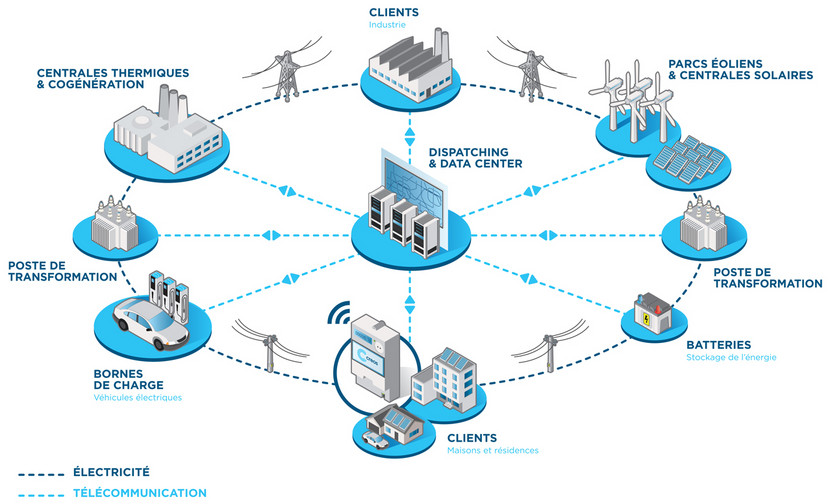
\includegraphics[scale=0.25]{media/smart_city_lux.jpg}
    \caption{
        Architecture d'une smartgrid\newline
        \tiny{Source: \url{https://www.creos-net.lu/creos-luxembourg/innovation/smart-grid/reseau-du-futur.html}}
    }
\end{SCfigure}

% Micro grid

La microgrid est un autre type de réseau qui, contrairement à la smart grid, ne s'occupe pas de la communication.
Cette solution est envisagée plus sérieusement par de nombreuses communes pour des raisons de coût, en effet, ses
avantages restent nombreux tels que la gestion de différentes sources d'énergies opérée de manière parallèle,
ainsi qu'une fiabilisation du réseau déjà présent.

% https://www.researchgate.net/post/What_is_the_difference_between_a_microgrid_and_a_smartgrid
% A microgrid is an electrical system that includes multiple loads and distributed energy resources that can be operated in parallel with the
% broader utility grid or a Small, independent power system. It Increased reliability with distributed generation, Increase efficiency
% with reduced transmission length, and Easier integration of alternative energy sources.while
% A smart grid is a modernized electrical grid that uses information and communications technology to gather and act on information,
% such as information about the behaviors of suppliers and consumers, in an automated fashion to improve the efficiency, reliability,
% economics, and sustainability of the production and distribution of electricity. Transmission and operations: wide‐area monitoring,
% control and protection.


% Analyse des villes

\section{Villes connectées}
% Cette partie parlera de la partie technique de la mise en place de la smart grid
%   Ainsi que des différents problèmes que les villes actuelles ont.

\section{Connectivité et population}
% Cette partie parlera de la partie humaine de la connexion a la smart grid.
% ex. La 5G (6G) et les réseaux sociaux
%     Communication et report de problèmes

\section{Les mutations de la ville}



\section{Étude de cas - IssyGrid}
Le projet IssyGrid® a été initié en 2012 par Bouygues Immobilier dans la ville d'Issy-les-Moulineaux,
commune française dans le département des Hauts-de-Seine. Le projet a été fortement encouragé par le
maire de la commune, André Santini. Mais aucun soutien d'ordre financier.

``La ville n’a pas mis un euro'' --  Éric Legale, directeur d’IssyMedia, chargé de la communication et
de l’innovation de la ville.

Le projet n'a pas impliqué qu'un seul acteur, mais un consortium de dix compagnies :
Bouygues Energies \& Services, Bouygues Immobilier, Bouygues Telecom, EDF, EMBIX, ENEDIS,
Microsoft, Schneider Electric, Sopra Steria et Total.

L'expérience a duré 6 ans, de 2012 à 2018, et a un impact sur la vie de 5.000 habitants, 10.000 employés
et 160.000 m2 de bureaux sur deux quartiers de la ville, Bords-de-Seine (quartier des affaires),
puis Fort en 2015.

Le projet a fait face à plusieurs types de défis. Tout d'abord des défis techniques.

Les habitations concernées ont été équipées d'un Linky, un compteur électrique conçu par EDF
plus intelligent que les anciens. Il est capable de suivre et de communiquer la consommation en
électricité tout comme son cousin Gazpar pour la consommation de gaz. La création de ces appareils répond
à une directive européenne, mais ils ont utiliser les Eco-quartiers comme terrain de test.
Total a également fait des progrès sur le raccordement des panneaux photovoltaïques.
L'énergie créée en trop lors des heures creuses est stockée dans des volants d'inertie et dans des
batteries. un accord a été passé avec Renault pour récupérer leurs anciennes batteries de voitures
électriques, démontrées comme suffisantes pour les quartiers Isséens.
Bouygues Energies \& Services a également travaillé sur l'éclairage urbain pour que les réverbères
consomment moins d'énergie et lutter contre la pollution lumineuse. Ils sont capables d'adapter
leur éclairage en fonction de l'heure et des présences à proximité.
Les données transitent dans toute la Smart Grid au travers d'un réseau développé par Embix, une
start-up créée par Bouygues. Ils ont livré le centre d'analyse et d'optimisation de l'ensemble des
flux énergétique, capable de communiquer avec tous les instruments de mesure du quartier, avec autant de
protocoles différents.

Mais aussi un défi concernant la récolte et l'utilisation des données utilisateurs.

Les informations de consommation d'énergie et de déplacements sont essentielles pour que la ville
puisse s'adapter à sa population. Le projet est parvenu à un accord sans précédent avec la CNIL :
la collecte des données est autorisée par lot de dix habitations afin de la garder anonyme, garantir
la confidentialité particulière d'un logement.
D'autant plus que la ville a choisi de faire de l'Open Data. Chaque foyer doit toutefois
donner son accord pour que ses données alimente le flux.

Un autre défi majeur fut la communication.

Tout au long du projet, la ville a fait un éffort de vulgarisation du projet afin de rassurer
la population par divers moyens de communication et de modules pédagogiques. La population a accès
a une interface pour suivre la consommation et la production d'énergie en temps réel grâce à des
graphes simples et intuitifs afin de la sensibiliser et la rendre actrice du projet.

Le projet IssyGrid inclus deux autres projets : SWAYS et SoMobility.

SWAYS - Smart ways to work - est un immeuble de travail de l'éco-quartier des affaires de IssyGrid.
Tout est fait pour le améliorer le confort des utilisateurs.
Il privilégie un éclairage naturel dans les bureaux et la purification de l'air par la biophilie,
le tout grâce à un toit végétale. Des commerces de proximité et autres structures de loisir
sont installés à l'intérieur même du bâtiment. D'un point de vue technique, le bâtiment serait
capable de d'anticiper les pannes grâce à de la maintenance prédictive, assure une couverture réseau
4G dans tout le complexe, et propose même aux utilisateurs des applications liées à l'activité du
bâtiment, ainsi qu'une cyber sécurité renforcée.

SoMobility est un projet dont le but est de fluidifier la circulation dans la ville. Les feux de
signalisation sont par exemple capables de prendre des initiatives pour optimiser le trafic.
Des applications proposent aux utilisateurs d'indiquer les places de parkings libres sur une carte.
Il y a actuellement un mini-bus qui se déplace sans chauffeur dans la ville.
Les données de circulation de ma ville sont encore une fois open data. Il est possible de visualiser
le trafic en temps réel sur plusieurs sites internet.
Au delà des ressources techniques mise en place, les habitants sont aussi sensibilisés à travailler
dans des espaces de coworking avant d'aller au bureau afin de désengorger les routes et transports
en commun, et le covoiturage est aussi mis en avant.

Le bilan de IssyGrid a été présenté en juin 2019.
Il ne présente malheureusement pas de chiffres pour ces six années de test, mais annonce en revanche
ses objectifs pour 2020 : ``Une efficacité énergétique accrue de 20 \%, une réduction de 20 \%
de l’empreinte carbone et une part de 20 \% des énergies renouvelables dans la production
énergétique européenne.''
La ville d'Issy-les-Moulineaux souhaite agrandir la Smart Grid à un troisième quartier
``Issy Coeur de Ville''. La ville de Nanterre s'inspire de ce projet pour lancer un projet
d'éco-quartier également.
Les chiffres d'IssyGrid n'ont pas été communiqués, mais un témoignage de Gironde HABITAT nous indique
que l'économie générée sur la consommation énergétique serait au mieux de 60€ par an à l'échelle d'un
foyer.

\section{Interview de M. Alexandre Capelle – Embix}
Nous avons pris contact avec M. Alexandre Capelle, Directeur des Solutions Logicielles chez Embix pour
lui poser quelques questions sur le projet IssyGrid.

Il a souhaité avant tout faire une mise en contexte :

\textbf{Alexandre C.} :
L'objectif de ce projet était d’expérimenter la connexion d’un morceau de ville à internet.
Il y avait trois défis : la collecte de données par l’installation de capteurs,
la récupération de données sur internet et le développement d’outils logiciels capables de traiter ces données.
Ça a pris la durée sur tout le long du projet. Tout d’abord dans le quartier des affaires,
là où sont implantés la majeur partie des entreprises d'Issy-les-Moulineaux – dont Bouygues Immobilier.
Puis le projet a été étendu aux nouveaux quartiers résidentiels dans un second temps.

\textbf{Quel a été l’impact de la smart Grid sur les entreprises présentes dans la Smart Grid ?}

\textbf{Alexandre C.} :
Ça n’a pas réellement changé leur façon de vivre, mais leur confort s'est amélioré.
Prenons l'exemple du siège de Bouygues Immobilier, dans le bâtiment Galéo. 
Il y avait peu de visibilité sur ses consommations énergétiques
et ses factures sans instrumentation pour mesurer ses performances énergétiques.
Le projet a permis de mettre en place les capteurs nécessaires pour remédier à ce problème.
Ils connaissent maintenant leur consommation et l’état de santé de leur bâtiment en temps réel.
Ils ont repéré pas mal de dysfonctionnements dans leur consommation.
Notamment sur le plan thermique, avec des température dont le réglage était incorrecte
et des fuites de chaleur aux niveaux de vannes qui devraient se fermer automatiquement.
Le confort pour les occupants n’était pas forcément assuré.
D'autres capteurs pour mesurer la qualité de l’air ont montré qu'elle se dégradait dans les salles de réunion après un certain temps.
L’objectif principal de la Smart Grid pour ce bâtiment était de pouvoir évaluer la performance
et le confort afin de pouvoir prendre les décisions pour corriger ces dysfonctionnements.
On navigue à l’aveugle sans ces outils logiciels.
Il est compliqué d’estimer le véritable gain monétaire, ou de performance,
mais le bien apporté au niveau du confort n’est pas négligeable du tout.

\textbf{Comment étaient gréffés les objets connectés au réseau ?}

\textbf{Alexandre C.} :
Alors il y a eu plusieurs types de capteurs.

Tout d’abord sur les bâtiments du tertiaire.
Aujourd’hui l’instrumentation est faite de manière systématique sur les bâtiments neufs.
Ils sont équipés de capteurs qui ne discutent pas directement sur Internet,
mais qui sont reliés entre eux au sein d’un réseau filaire avec des protocoles de communication
tels que Modbus, BACnet, qui permettent de communiquer via des câbles ethernet ou Modbus
et de partager leurs informations entre eux.
Derrière il y a des outils logiciels, communément appelés GPB (Google Protocol Buffers) qui accèdent à ce réseau
pour interfacer en temps réel les données de tous les capteurs.
C'est le GPB qui fait la connexion à Internet pour rendre visibles ces données depuis l'extérieur.
La mise en place du réseau a été livré en même temps que les bâtiments.
Mais pour avoir accès à l’information par Internet il a fallu quelques travaux en plus. 

Le fonctionnement est différent dans les bâtiments d'habitation.
Dans chacun des 600 logements, il y a eu un gros compteur installé
auquel est relié tout un réseau de capteurs capables de lui transmettre l’information en filaire :
température, consommation de chauffage, consommation électrique\dots
Le compteur, lui est connecté directement à Internet. 

La Smart Grid récupère aussi des informations via des objets connectés dans la ville,
notamment sur la Gare SNCF, Val-de-Seine (RER C).
Il y a un objet connecté posé directement sur le compteur ENEDIS pour mesurer la consommation électrique via un réseau longue porté, LoRa.
Il s’agit d’un réseau déployé par Bouygues Telecom qui couvre tout le territoire français en passant par les ondes radio.
Le maillage en France est de l’ordre du kilomètre.
Ces objets connectés compatibles LoRa peuvent donc communiqués en utilisant ces antennes là.
La données est ensuite stockée sur les serveurs de Bouygues Telecom.
L’avantage est qu’il n’y a pas de câble, ce qui est très pratique pour l’installation. 

Les réseaux électriques et thermiques sont gérés par ENEDIS.
Ils équipent les appartements récents des compteurs Linky leur permettant de récupérer à distance les données de consommation.
Les données journalières sont automatiquement enregistrées sur les serveurs ENEDIS.
Avec l’accord du consommateurs, il peut faire un enregistrement toutes les 30 minutes.
N’importe quel acteur qui dispose du consentement de l’abonné au réseau peut récupérer la donnée de consommation énergétique auprès de ENEDIS.
Dans le cadre d’un projet urbain par exemple.
Mais il n'est pas possible de communiquer directement avec les compteurs.
Le rôle d'Embix était donc d'assurer la collecte de données et le développement des interfaces pour voir ces données. 

\textbf{Y avait-il d'autres capteurs en ville ? Pour gérer le trafic au niveau des feux rouges par exemple ?}

\textbf{Alexandre C.} :
Dans une rue du le quartier d’affaire, il y a des capteurs au niveau de l’éclairage public.
On récupère la donnée à distance pour savoir si un éclairage est allumé ou non.
L’échange est bidirectionnel, on peut envoyer un signal au luminaire pour qu’il s’éteigne par exemple.
Il y a aussi des capteurs de présence pour les piétons et véhicules, pour ajuster l’éclairage public et n’éclaire qu’en cas de besoin.
C’est à dire lorsqu’il y a un piéton ou véhicule en approche.
L’éclairage n’est pas totalement éteint, on ajuste la puissance de l’éclairage de la rue.
S’il n’y a personne, on réduit l’intensité lumineuse.
On a pu diviser par 2 la consommation de l’éclairage public avec ce système.
Ça n’a pas été compliqué à mettre en oeuvre et le résultat était immédiat. 
Il y a eu des sujets autour de ces luminaires pour en faire des points relais wifi, mais ce projet n’a pas abouti. 
L'exemple que vous avez cité – la gestion du trafic par les feux tricolores) n’a pas été implémenté dans IssyGrid.
Il y a des villes plus connectées que d’autres, Montpellier, Dijon, Angers, qui investissent beaucoup dans ce domaine.
Ils proposent par exemple des données permettant de trouver des places de parking disponibles.
Des capteurs de présence et de géolocalisation relèvent les places de parkings disponibles
et permettent d’alimenter des applications pour relayer l’information à la population avec un mapping des places de parkings.
Il me semble qu’il y a des applications de ce type là à Nice ou Lyon. 
Mais on est plus dans de la Smart City que de la Smart Grid.
L’utilisation de ces données là dans une Smart Grid a pour but l’économie d'énergie :
électricité, chaleur, consommation d’eau également\dots 

\textbf{Est-ce que la Smart Grid a permis à la ville d’avoir un mix énergétique un peu plus vert ?}

\textbf{Alexandre C.} :
C’est une sacré question, et vous n’aurez pas la même réponse selon l’interlocuteur. 
Il y a plusieurs périmètres.
D’une part à l’échelle du territoire international, il y a un besoin d’équilibrer la consommation d’électricité et sa production.
La personne morale responsable de ce niveau est RTE (Réseau de Transport de l’Electricité), une entreprise française semi-publique.
Sa mission est d’équilibrer production et consommation grâce à de l’analyse prédictive de la consommation en électricité
de l’heure suivante à 1\% près sur le territoire français.
Elle s’appuie sur les productions des centrales nucléaire, mais également de plus en plus de production renouvelables : photovoltaïque, éolien\dots
Mais les énergies renouvelables posent un défi supplémentaire puisque leur production est intermittente,
à cause de la météo notamment, contrairement à la centrale nucléaire où la production est à la demande.
Une Smart Grid à l’échelle nationale est capable de prédire ces données météo pour adapter la distribution en temps réel.
Il y a quelque chose de très bien développé en France qui est l’effacement.
Les gros consommateurs d'électricité comme des industriels se mettent d’accord entre eux et avec le réseau
pour ne plus consommer pendant un laps de temps.
Par exemple, RTE détermine que la consommation en France à 19h va être très élevée
et qu’elle n’est pas capable de répondre à la forte demande considérant son nombre d’unités de production.
Elle va donc demander à de gros consommateurs d’arrêter de consommer pendant une courte période.
La Smart Grid permettrait donc de faire ces analyses et ses demandes d’effacement de façon automatique. 
Plus on utilise d’énergie renouvelable, plus on a besoin de recourir à cette politique d’effacement 
car la production est moins prévisible et nous deviendrons dépendants des ces logiciels là. 
A l'échelle de la collectivité, les volumes de production installés dans les communes
n’est pas encore assez important la plupart du temps pour poser problème.
Dans le cas d’une petite ville qui aurait fait le choix de grand parcs d’énergies vertes,
il faudrait construire le projet avec ENEDIS qu’il n’y pas de soucis particulier dans le réseau.
A ce jour, je n’ai pas vu de genre de “réel” Smart Grid. 
Mais je l’ai vu sur des espaces privés.
Nous avions un projet sur le site du siège social de Bouygues Construction du coté de Saint-Quentin-en-Yvelines.
C’est une petite ville avec entre 1 000 et 5 000 personnes qui travaillent.
C’est un territoire privé, donc il est possible de réaliser des optimisations énergétiques à cette échelle.
Sur un territoire public, les optimisations de réseau sont déjà faite par RTE et ENEDIS,
donc il n’y a pas trop d'intérêt à optimiser une deuxièmes fois la consommation.
C’est déjà de leur responsabilité et par extension celle de l’État. 

\textbf{Ce n’est donc pas à la Smart Grid de gérer l'équilibre, son but est d’informer RTE qu’un équilibre peut être rompu ?}

\textbf{Alexandre C.} :
Oui c’est un peu ça. Smart Grid est un mot qui peut désigner beaucoup de choses.
Mais à partir du moment où on manipule de l’information on est déjà en train de faire du Smart Grid. 
Le deuxième avantage de la Smart Grid est de pouvoir mapper le réseau et détecter les dysfonctionnements en temps réel
quand une alimentation électrique est coupée pour intervenir immédiatement. 

\textbf{J’ai vu qu’il y avait pas mal de nouvelle technologies qui venaient de voir le jour justement pour rééquilibrer les périodes creuses.
Des petites unités d’hydrogènes qui se mettaient proches des énergies intermittentes.}

\textbf{Alexandre C.} :
On peut parler du stockage un peu de manière générale.
C’est une manière différente de contribuer à l’équilibre entre offre et demande.
Si on a trop de production photovoltaïque, on peut stocker sous sous forme de batterie,
soit sous forme d’hydrogène, ou d’une autre manière l'énergie excédentaire pour la restituer plus tard.
Les grosses centrales photovoltaïques sont couplées avec du stockage afin de pallier à cette intermittence.
Les systèmes de stockages peuvent contrebalancer les déséquilibres dus à la météo afin de lisser la production et mieux prévoir la quantité produite.
Les batteries permettent aussi de faire de l’effacement.
On stocke au moment où l’électricité est pas chère et la libérer lorsque le réseau en a besoin, au moment où le coût de l’électricité est plus élevé.
Avec l'excédent de production on peut aussi fabriquer de l’hydrogène.
Soit on utilise ensuite l’hydrogène tel quel et le revendre à des industriels, par exemple dans de stations service de véhicules à hydrogène.
On peut aussi restituer l’électricité à partir de l’hydrogène et s’en servir comme d’une batterie. Tout cela est encore expérimental,
on n’a pas encore trouvé de véritable modèle économique. Et les coûts sont encore trop élevés pour que ça puisse fonctionner à grande échelle.


\textbf{Comment se sont rassemblés tous les acteurs du projet ? Y-a-t'il eu un appel d'offre ?}

\textbf{Alexandre C.} :
L’impulsion initiale a été lancée par Bouygues et la ville, mais le projet a été lancé par tous les partenaires.
Ce projet est particulier dans le sens où il a été financé par les partenaires du projet.
Les entreprises du consortium ont toutes investi la somme de 250 000€ – si je ne me trompe pas.
Bouygues Energies \& Services, Bouygues Immobilier, General Electric, EDF, ENEDIS, Microsoft, Objenious, Schneider Electric, Sopra Steria et Total.
Les plus gros acteurs industriels ont décidé collectivement d’expérimenter là dessus pour voir quels seraient les gains réalisés dans ce domaine.
Pour se rendre compte des difficultés qui pourraient être rencontrées notamment en terme de collecte de données.
Il n’y a pas eu d’appel d’offre, de sélection pour créer ce projet là.
Ni de subvention particulière, c’est de la R\&D.
Derrière il y avait des partenaires du projet comme Embix ne faisant pas partie du consortium car ils n'avaient pas fait d’apport budgétaire.
Le pot commun a permis de financer les travaux. Il a été utilisé pour faire travailler des entreprises comme la nôtre.
Embix a été créé en 2011 à l’occasion de ce projet par des membres du consortium,
les trois actionnaires de l’époque : Bouygues Immobilier, Bouygues Energie et Service, et General Électric,
anciennement Alstom Grid – ils ont été rachetés depuis.

\textbf{Embix a donc eu d'autres projet après IssyGrid ?}

\textbf{Alexandre C.} :
Aujourd’hui, General Electric n’est plus dans notre actionnariat. Il ne reste plus que Bouygues Immobilier, et Bouygues Électrique et Service.
On travaille sur une quarantaine d'autres projets – à des stades de développement divers – maintenant que IssyGrid est terminé.
On a pas mal de projets à Paris, plusieurs à Lyon aussi, quelques villes en France, on a un projet au Maroc, un autre sur l’Ile Maurice\dots
On commence à avoir pas mal de choses en France et à l’international en somme.
Chacune des villes a sa problématique, mais on retrouve un même besoin partout qui est de suivre la consommation énergétique.
Ils renouvellent le parc immobilier en créant de nouveaux quartiers et en promettant des quartiers éco-responsables.
Mais quand on mesure – si on mesure – on se rend compte que les performances énergétiques ne répondent pas aux critères énoncés initialement.
Notre rôle est d’instrumenter le quartier pour récupérer de la donnée, regarder la performance et la comparer avec ce qui était prévu.
Puis apporter les corrections nécessaires pour que le quartier fonctionne correctement.
Comme je le disais tout à l’heure, chacun a sa définition de la Smart Grid.
La seule chose en commun entre toutes ces définitions est la notion de préservation de l’énergie et la collecte des données.
Ce qu’on en fait ensuite dépend de celui qui la manipule, chacun apporte sa pierre à l’édifice.

\textbf{Vous êtes-vous inspirés d’autres projets de Smart Grid lors de l’instruction du projet d’IssyGrid ?}

\textbf{Alexandre C.} :
Les personnes qui intervenaient dans le consortium avaient par le passé participé à d’autres projets.
En France pas vraiment, puisque IssyGrid est une première.
Il y a eu des projets démonstrateurs un peu avant, sur des périmètres contrôlés.
Il y a eu un projet qui a fait un peu parler de lui, Nice Grid.
L’inspiration du projet a pu venir des États-Unis et d’Angleterre.
Mais le fonctionnement est là-bas, les réseaux de transport et de distribution sont des acteurs privés.
Ils se permettent d'aller un peu plus loin dans l’optimisation énergétique et proposent des choses plus innovantes.
L’un des freins à la Smart Grid en France, puisque c’est public,
les infrastructures sont sur-dimensionnés pour éviter toute coupure électriques – ou presque.
Pour que le réseau ne tombe pas chez nos voisins anglais ou allemand, ils ont besoin de plus de surveillance.
Les Smart Grids sont donc plus développées dans ces pays là.
Les choses tendent à évoluer en France car l’État commence à être plus regardant sur les dépenses de ENEDIS et RTE,
et demande de moins surdimensionner et de mieux équilibrer offre et demande.
On rentre dans des discussions assez politiques du fait que le réseau soit public malheureusement.
Le fonctionnement du réseau en France impacte les projets de Smart Grid.
C’est donc un frein au développement de l’activité en France et je pense que mon avis est partagé par les acteurs du secteur.
Pardon, je crois que je me suis écarté de la question.
Nous avons surtout appris au cours du projet, il a quand même duré 8 ans !
Ce genre de projet démonstrateur et R\&D dure d'ordinaire 3 ou 4 ans.
Ce sont surtout les autres projets qui se sont inspirés d’IssyGrid et non l’inverse.
Il a beaucoup rayonné dans le monde. On a encore aujourd’hui des délégations chinoises ou japonaises.


\textbf{Quels enseignements avez vous pu tiré de ce projet au cours de ces 8 années, et quelles étaient les quick win
– les actions mises en place avec peu d’effort mais à forte valeur ajoutée ?}

\textbf{Alexandre C.} :
La collecte de données a été complexe en l’absence de standardisation.
Les capteurs utilisés sur les bâtiments et par chaque fournisseurs sont différents et communiquent par des protocoles tout aussi différents.
Nous avons dû apprendre à communiquer avec une quinzaine de protocoles différents afin d’agglomérer l’information en un endroit
et de la rendre accessible via une interface.
C’est plus rapide à apprendre qu’une langue vivante mais parfois dans certains cas ça reste un vrai défi.
Il n’y avait pas vraiment de projets existants de cette envergure : 600 logements, 15 bâtiments tertiaire, une gare…
Ce qui représente beaucoup de types de données différentes.
Un de nos quicks win est sans doute l’éclairage public. Plusieurs villes font ça maintenant.
Il y a aussi eu quelques essais de stockage de froid dans un grand bâtiment.
Et je parle d’une grande tour, comme ce qu’on pourrait avoir à la Défense – je ne pourrais pas vous dire la taille exacte.
Cette grande tour a une consommation d’énergie conséquente, notamment l’été en pour faire tourner la climatisation.
La nuit – durant les heures creuses – on va volontairement consommer plus d’électricité pour fabriquer de la glace.
Et lorsqu’il y a des problèmes de chaleur vers 14h en semaine, plutôt que de faire fonctionner la climatisation,
on va laisser fondre ce bloc de glace pour produire de l’électricité. Ce bloc de glace est en fait utilisé comme une batterie.
Ce n’est pas très cher à mettre en place – à l’échelle du bâtiment – et à utiliser.
C’est intéressant puisque ces problèmes de climatisation et de consommation est un véritable sujet à la Défense,
et on pourrait réduire leur consommation en les équipant de ce système, et donc éviter de surdimensionner le réseau électrique.
Indépendamment du réseau, il y a un gain économique à ce stockage.

\textbf{Quelles seraient les différences entre un projet Smart Grid créé aujourd’hui et un projet dans 5 ans ?}

\textbf{Alexandre C.} :
Question difficile. Tout d'abord le projet ne serait pas initié par les mêmes personnes.
Au début d’IssyGrid, il n’y avait que peu de projets et peu d’acteurs. Et les projets consistaient surtout en de la R\&D.
Aujourd’hui, les quartiers de ce types seraient initiés par les promoteurs immobiliers.
Ils profitent de la construction de nouveaux quartiers pour bénéficier de ces technologies.
Une autre différence est qu’avant on mettait beaucoup l’accent sur la recherche de l’équilibre offre-demande avec de l’intelligence artificielle,
des algorithmes d’optimisation compliqués.
Il faudrait vraiment que le réseau locale présente des particularités pour mettre en place tous ces procédés.
Une station de ski par exemple, qui n’est alimenté que par une source.
Il y aurait un risque de coupure en électricité si la ville consomme trop.
Aujourd’hui on chercherait plutôt la tenue de la performance.
On s’est rendu compte qu’en instrumentant pour récupérer de la données que nos systèmes énergétiques
ne fonctionnent pas bien en France, car personne ne surveille.
Une Smart Grid s’attache a établir des objectifs de performance et apporter une solution technique pour suivre cette performance.

Nous remercions M. Alexandre Capelle d'avoir pris le temps de répondre à nos questions avec autant de détails.

\section{Des projets en échec}

Lors de la VivaTech Paris 2019, Emmanuel BAVIERE (Société Générale), Erwan KERYER (KPMG)
et Jérôme MONCEAUX (SPOON) ont pris la parole le vendredi 16 mai pour expliquer le phénomène autour des
Smart Grid. Un terme fort a été employé durant cette prise de parole :
``La Smart City ne marche pas''.

En se basant sur plusieurs exemples de projets en échec, divers arguments à ce propos ont été mis en
avant :
\begin{itemize}
    \item Des projets trop ambitieux ;
    \item Un manque de communication avec la population qui fait face à une puissance effrayante car mal comprise ;
    \item Les grands groupes ne savent pas comment gérer les tensions et désaccords avec les élus et la population ;
    \item Un manque de formation de la population qui ne sait pas utiliser les nouvelles technologies ;
    \item Une population qui refuse de partager ses données pourtant nécessaires au bon fonctionnement d’une Smart Grid ;
    \item Le gouffre séparant les populations aisées des populations pauvres s'élargie.
\end{itemize}

Le projet Quayside de Toronto réunit la plupart de ces éléments.
% Description du projet
Les oppositions au projet sont multiple. On lui reproche avant tout son manque de démocratie.
Bianca Wylie, une opposante au projet, accuse les grands groupes derrière le projet de vouloir noyer l'information
avec la publication d'un document aussi volumineux auprès de la population.